\chapter{Event preselection}\label{chap:preselection}
The experimental signature of our signal is the presence of two same-sign
prompt leptons and at least four jets (see figure~\ref{fig:TTbar_feynman}).

\begin{figure}[htb]
    \centering
    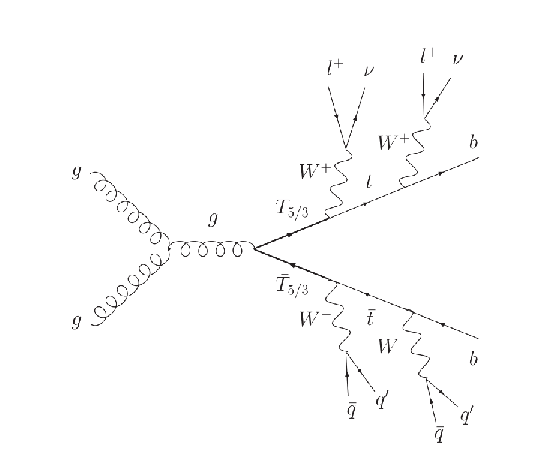
\includegraphics[width=\textwidth]{images/pdf/TTbar_feynman}
    \caption{Pair-production of the \TP, decaying into same-sign leptons and
    at least four jets.}
    \label{fig:TTbar_feynman}
\end{figure}

The backgrounds associated with this signal can be divided into three
categories:
\begin{description}\label{page:background_categories}
    \item[two same-sign prompt leptons] from rare SM processes.
    \item[opposite-sign leptons] whose charge is mismeasured, leading to a
        same-sign final state.
    \item[one prompt and one non-prompt lepton with the same charge] (or two
        non-prompt same-sign leptons). This background arises mainly from
        \ttbar events where one of the leptons comes from the decay of a
        $b$ quark, but is mistaken for a prompt lepton.
\end{description}

In order to reject all of these background sources, the following baseline
selection is applied:
\begin{itemize}
    \item event cleanup and trigger
    \item exactly two same-sign leptons, rejecting events with three or more
        leptons
    \item quarkonia veto, with the invariant mass of the leptons greater
        than \unit[20]{GeV}
    \item \Z veto, with the invariant mass of the \E\E and \M\M pairs not in
        the 76-106 window. This selection is not needed for \E\M
        events for lepton number conservation.
    \item at least four jets
\end{itemize}
The event cleanup and trigger requirements are detailed
in~\ref{sec:event_cleanup} and~\ref{sec:triggers}.
The invariant mass selections are particularly well suited to 
reject events with charge misidentification, in addition to the charge
consistency requirement on page~\pageref{page:electron_charge}, particularly from $\Z
\rightarrow \E\E$ decays. Figure~\ref{fig:lep_mass} clearly shows a peak at
around the mass of the \Z boson for the double electron channel. The effect
is much smaller for the muons. 
The distribution of the number of jets in the signal and backgrounds
(figure~\ref{fig:n_jets}) also
shows that this is a good discriminating variable against both the
prompt and the \ttbar backgrounds.

\begin{figure}[htb]
    \centering
    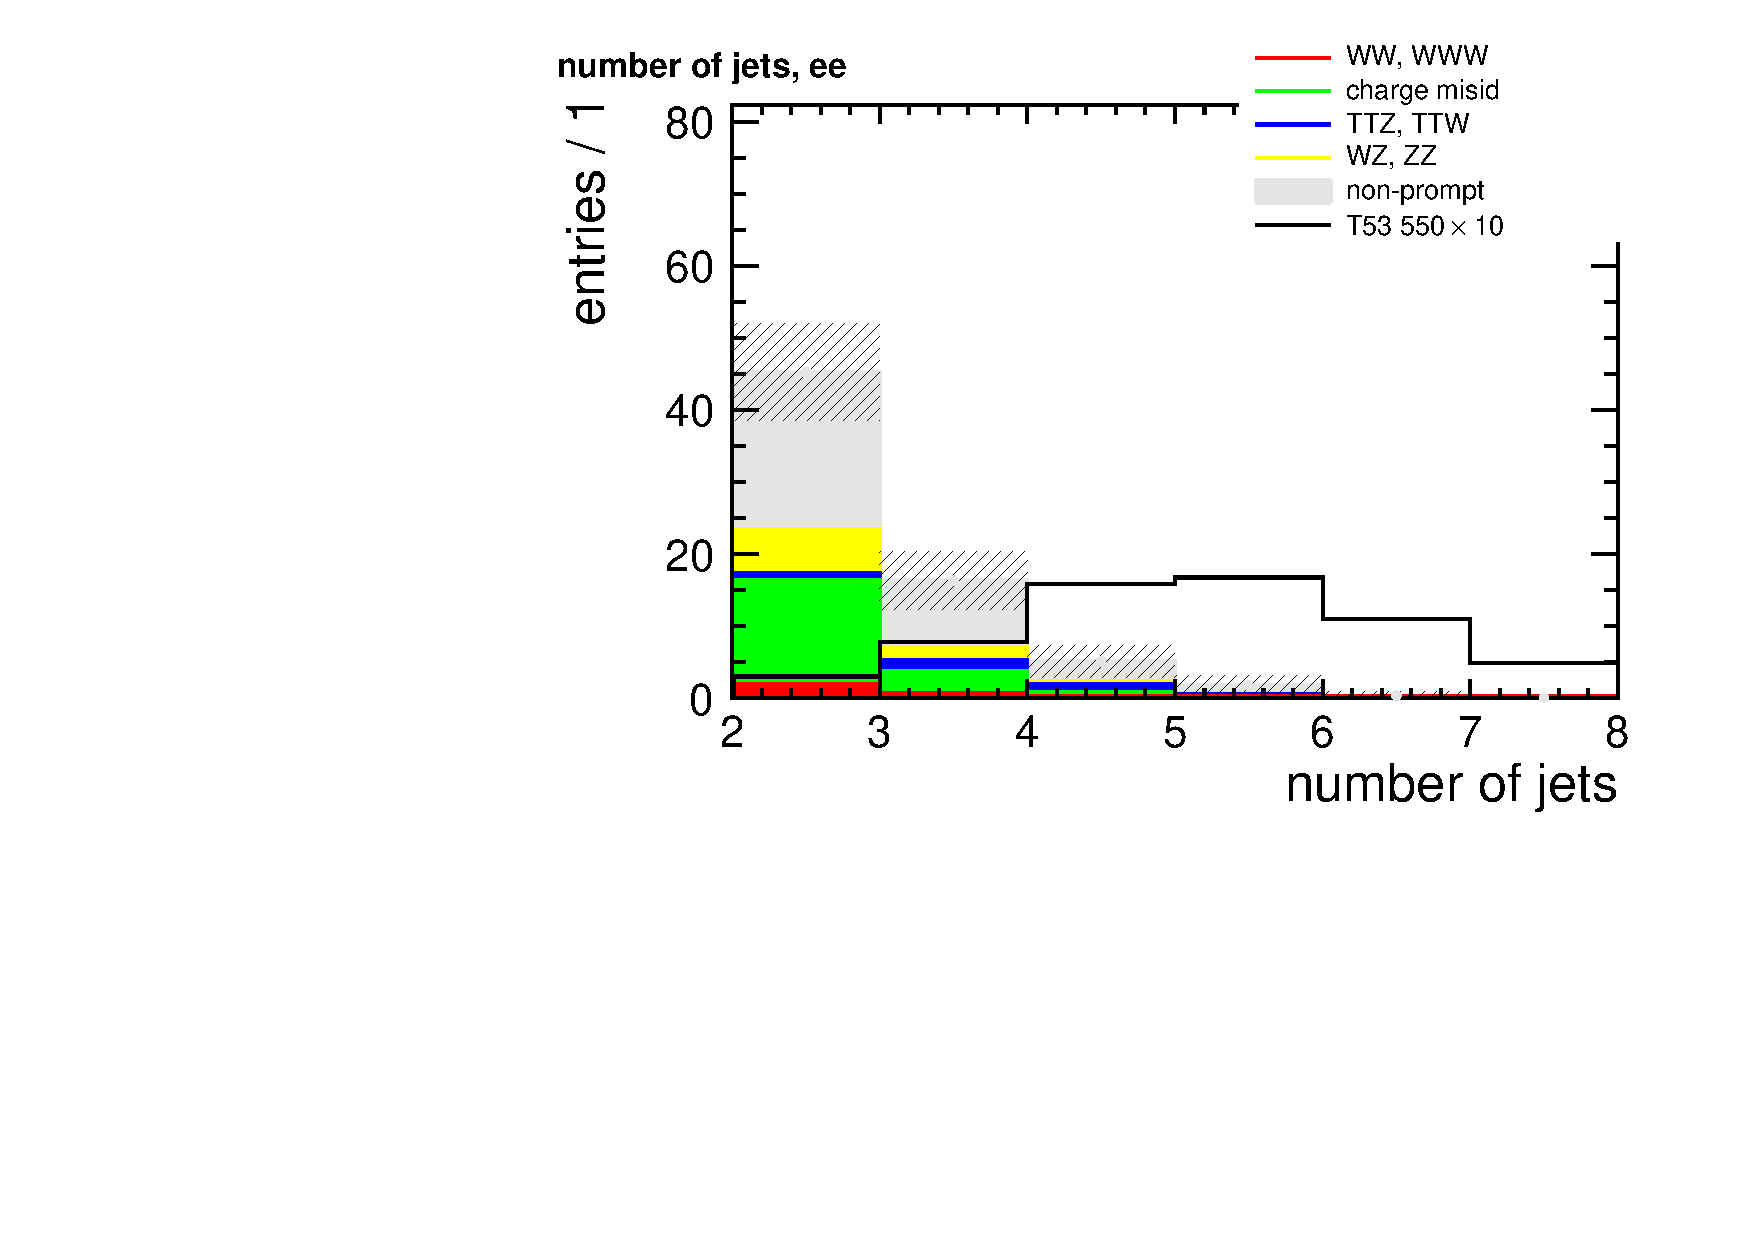
\includegraphics[width=.49\textwidth]{images/pdf/same-sign,_2_jets/n_jets_ee_0}
    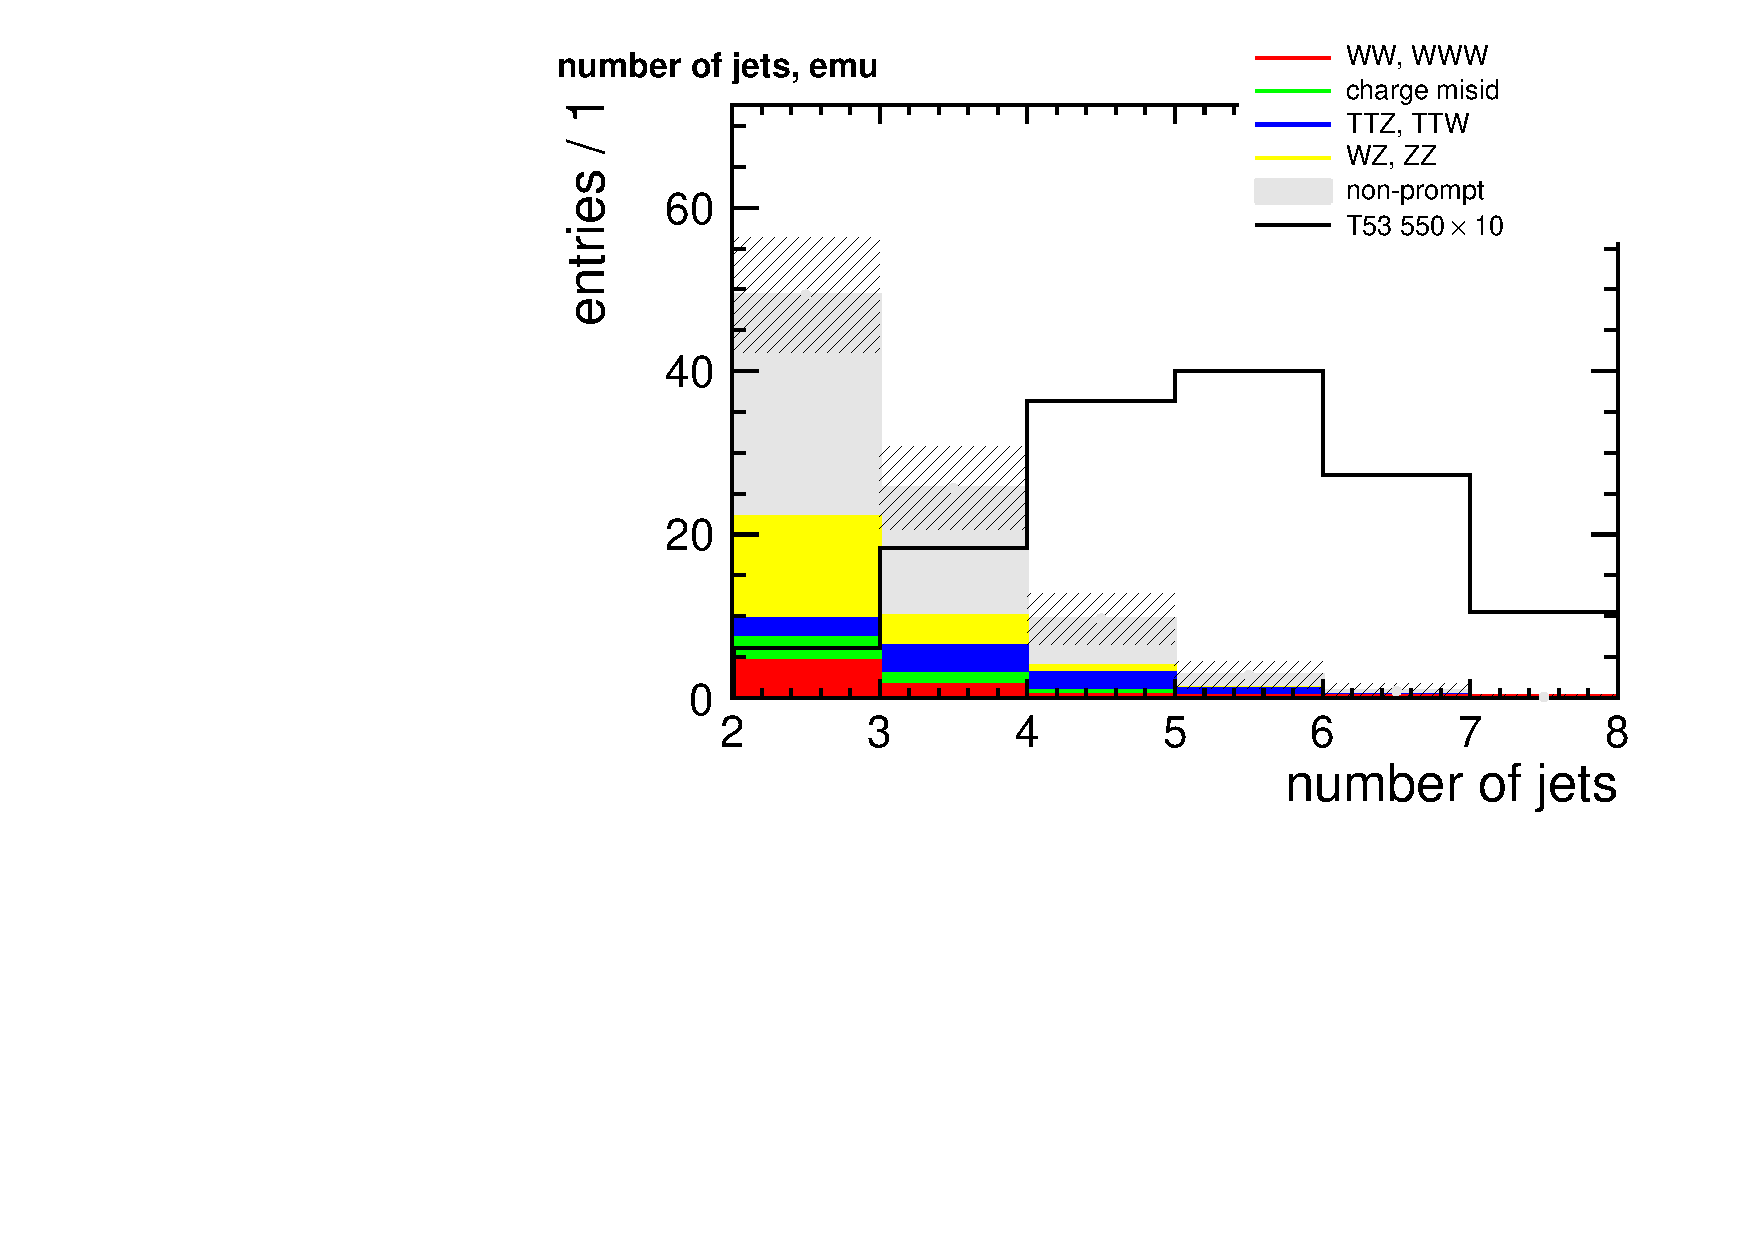
\includegraphics[width=.49\textwidth]{images/pdf/same-sign,_2_jets/n_jets_emu_0}\\
    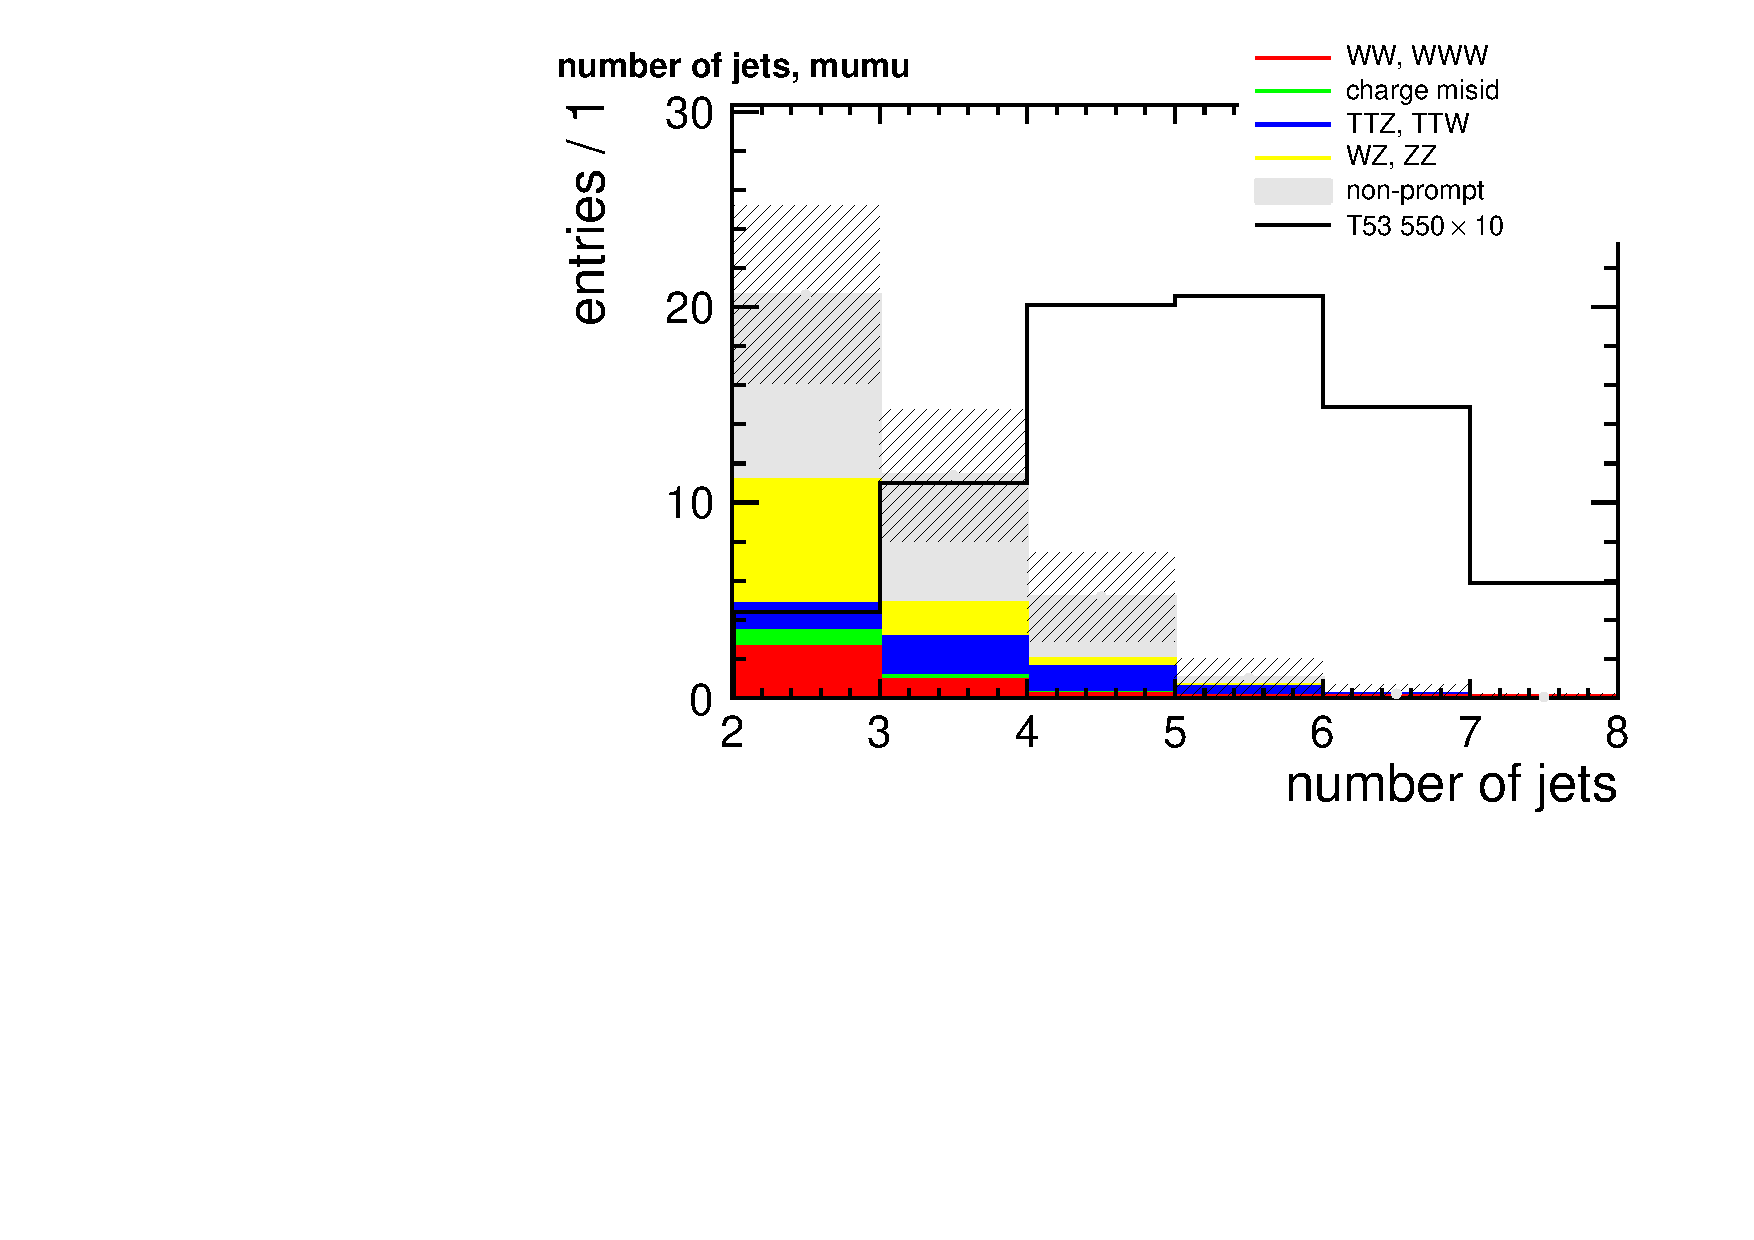
\includegraphics[width=.49\textwidth]{images/pdf/same-sign,_2_jets/n_jets_mumu_0}
    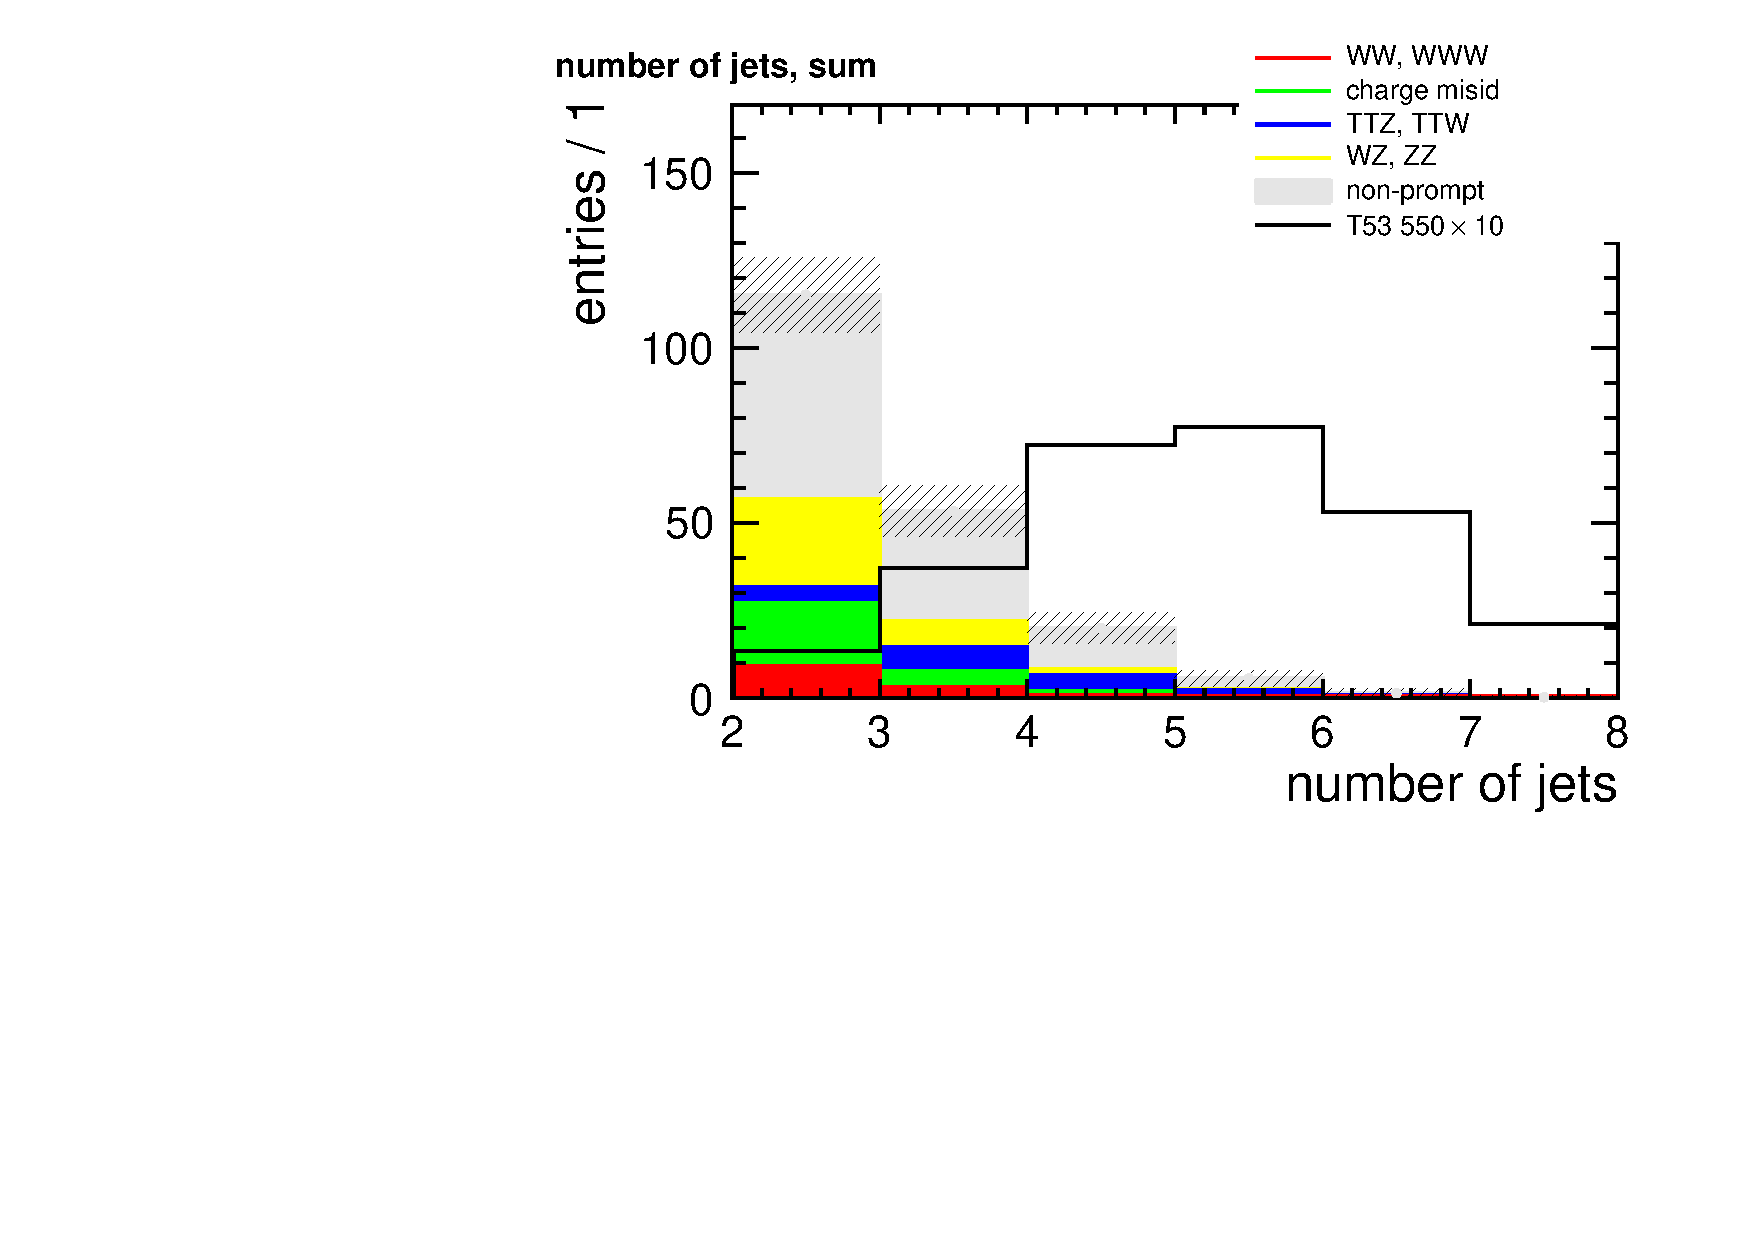
\includegraphics[width=.49\textwidth]{images/pdf/same-sign,_2_jets/n_jets_sum_0}
    \caption{Events with two same-sign leptons and two jets. Distribution of the number of jets in the backgrounds and
        signal for the \unit[550]{GeV} mass point for the sum of the three
        decay channels \E\E, \E\M\ and \M\M, and their sum. The signal is
    amplified by factor of ten, the data-driven backgrounds for the
non-prompt and charge misidentification contributions are detailed in
chapter~\ref{chap:data_driven}. The shaded area includes statistical and
systematic uncertainties.}
    \label{fig:n_jets}
\end{figure}

\begin{figure}[htb]
    \centering
    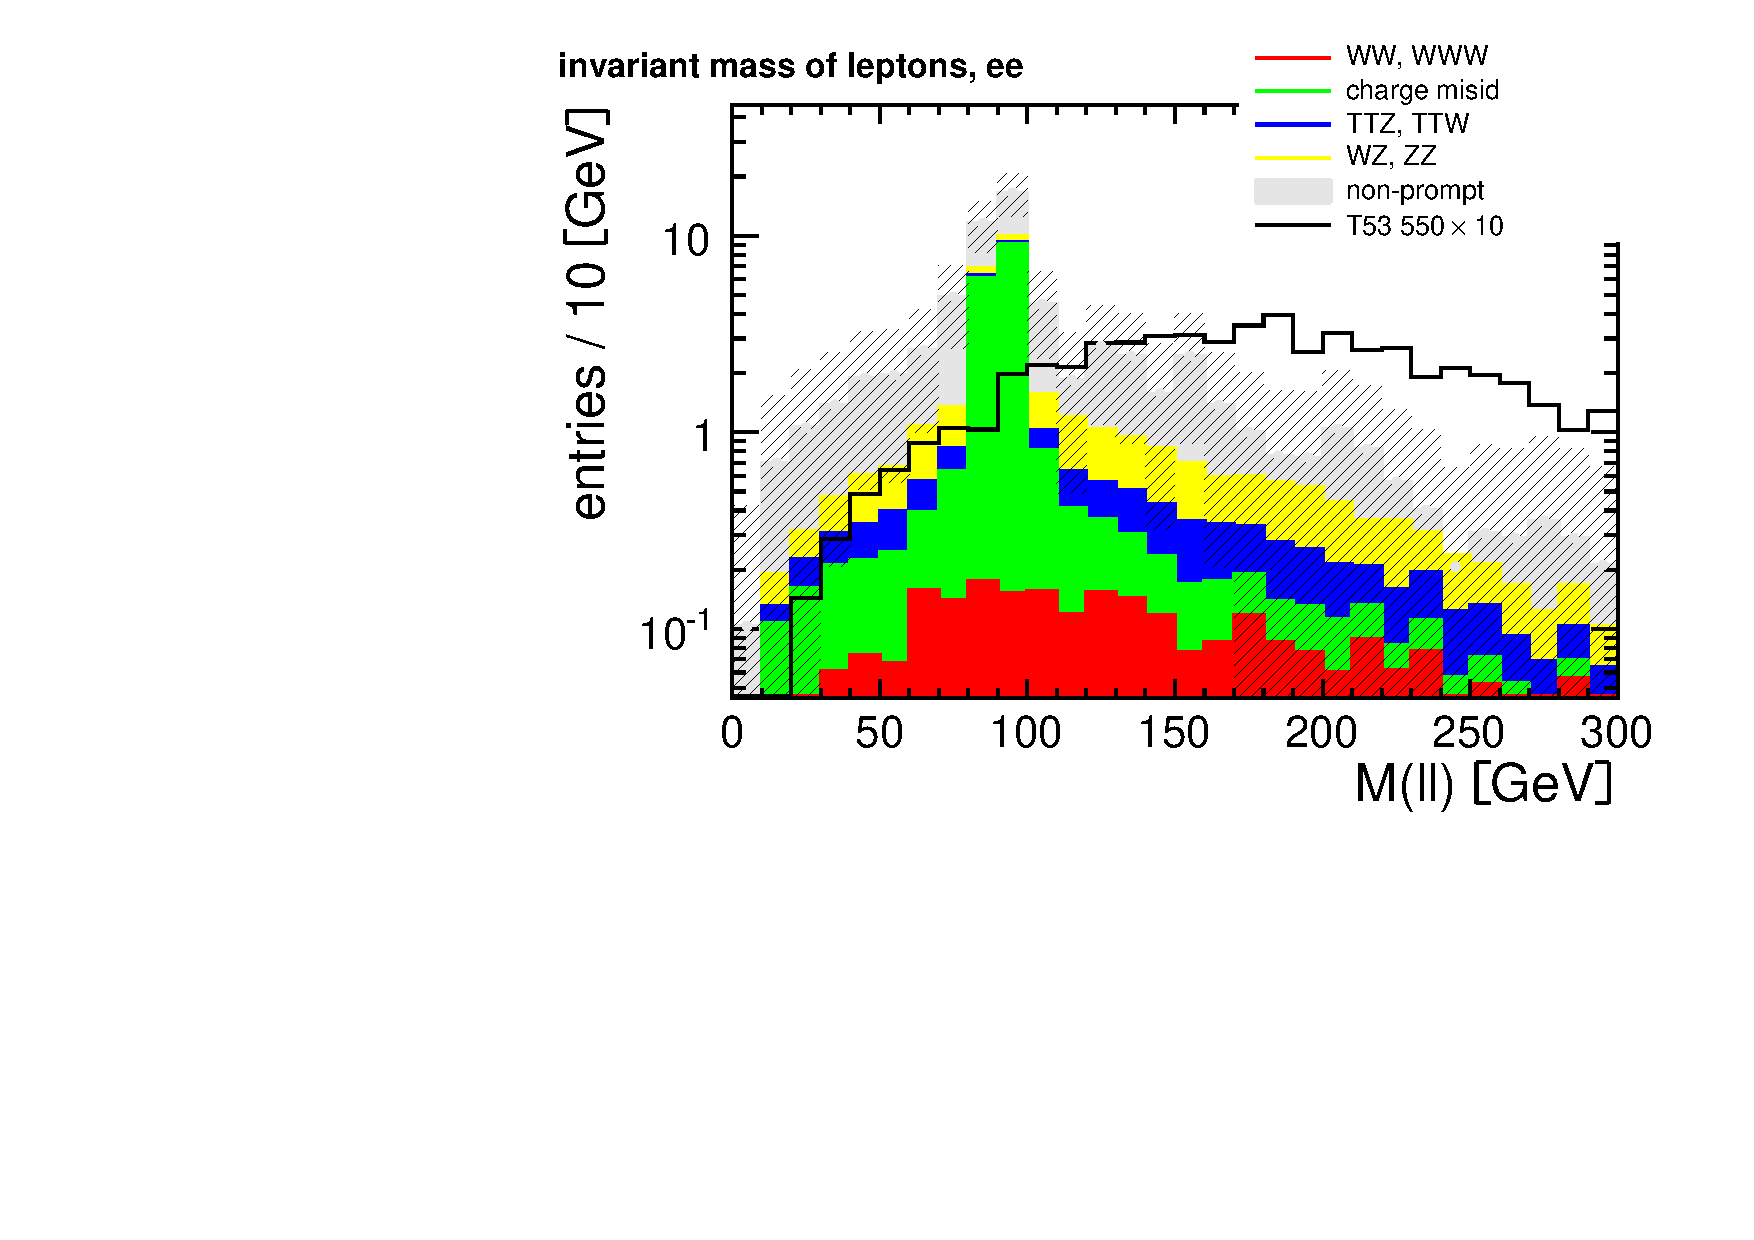
\includegraphics[width=.7\textwidth]{images/pdf/same-sign,_2_jets/lep_mass_ee_0}
    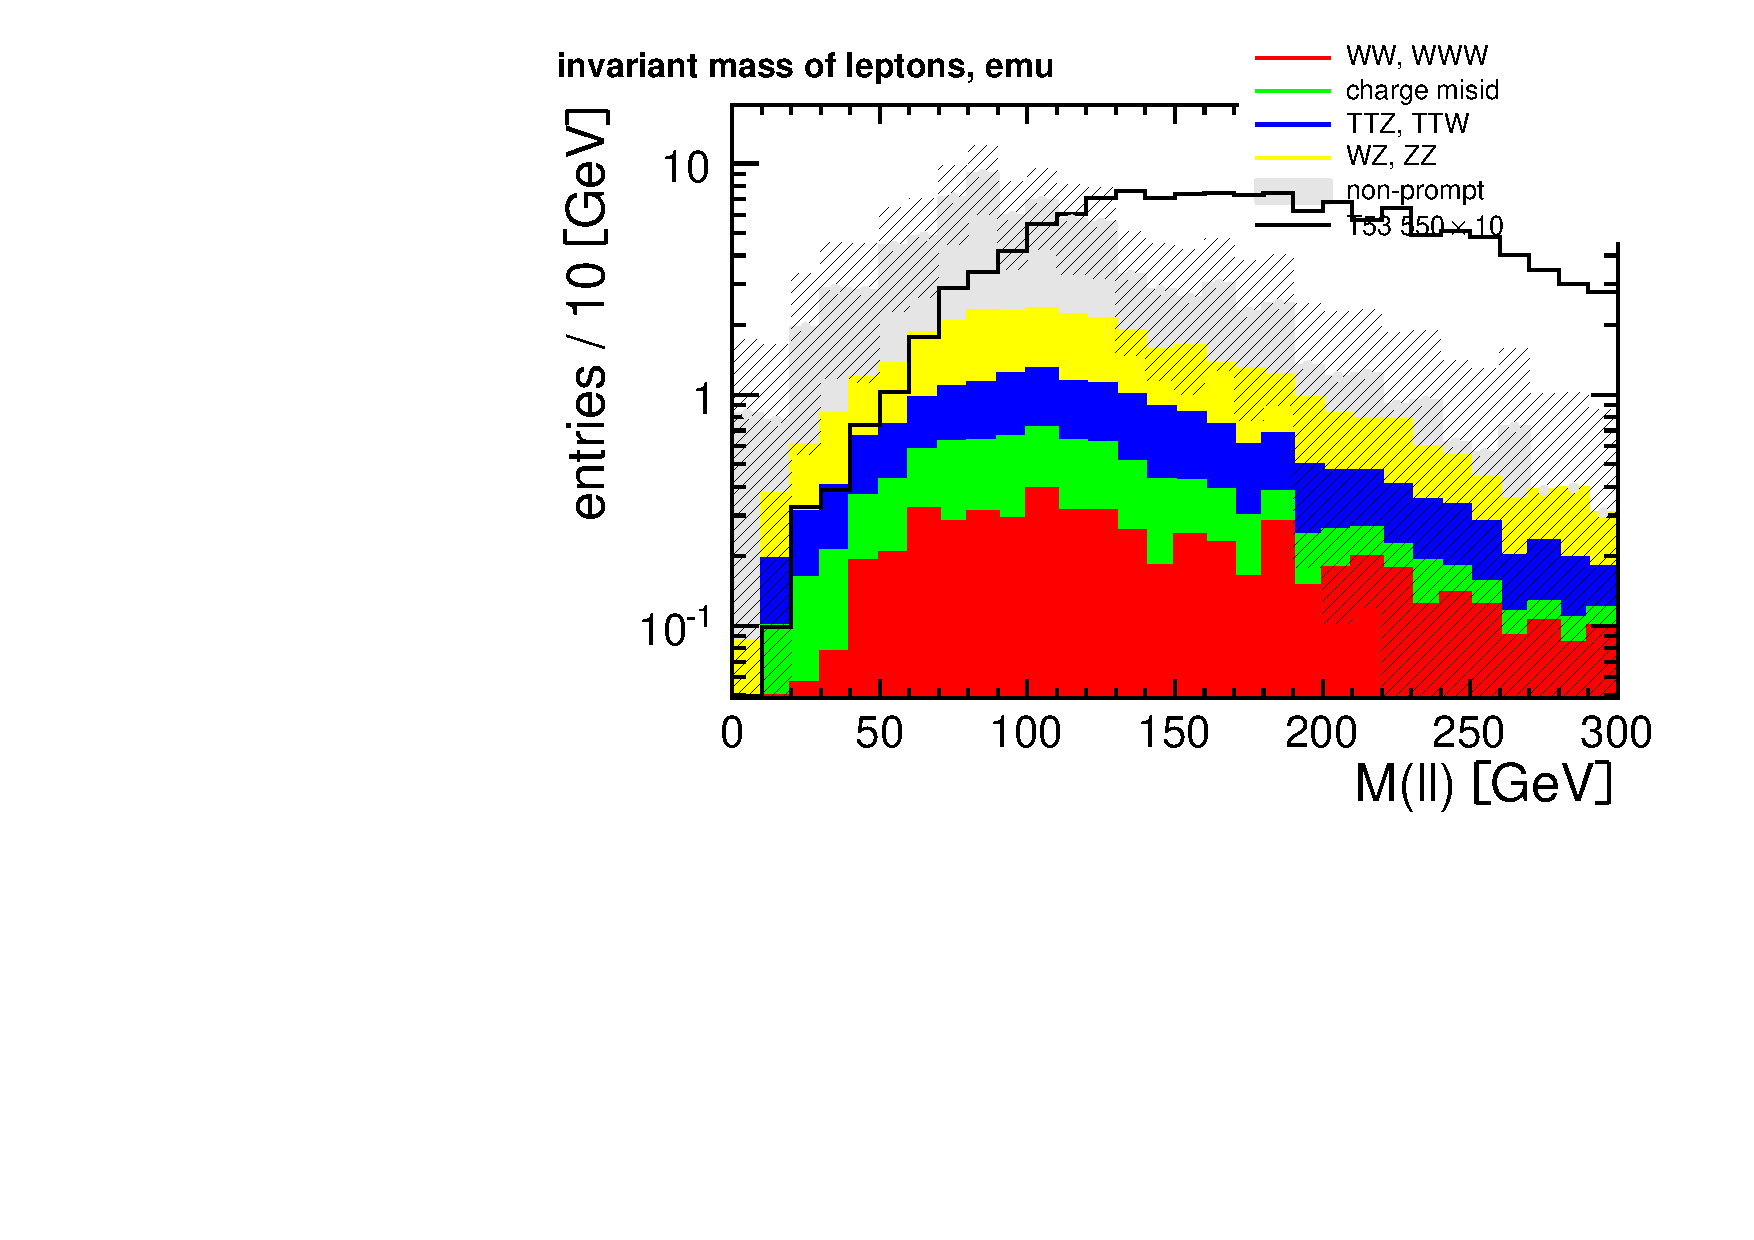
\includegraphics[width=.7\textwidth]{images/pdf/same-sign,_2_jets/lep_mass_emu_0}
    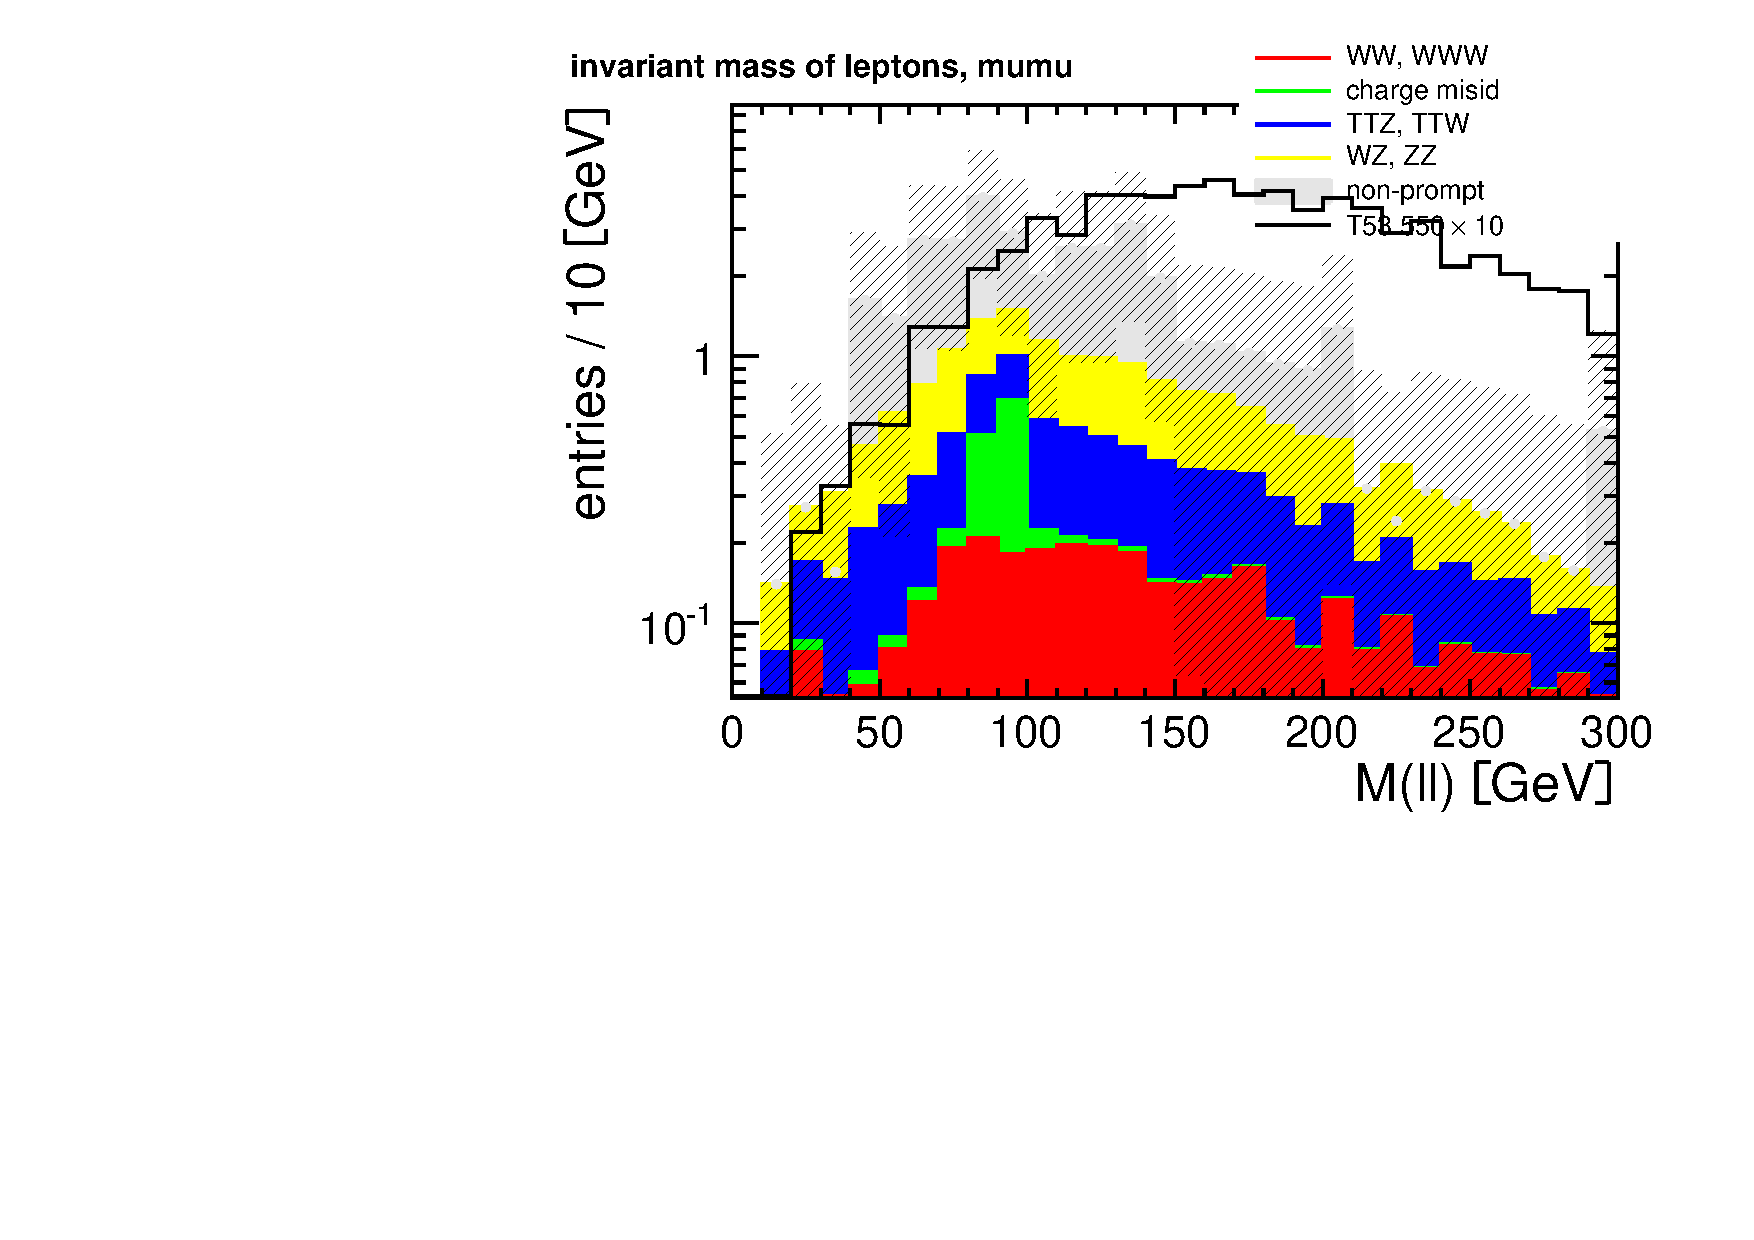
\includegraphics[width=.7\textwidth]{images/pdf/same-sign,_2_jets/lep_mass_mumu_0}
    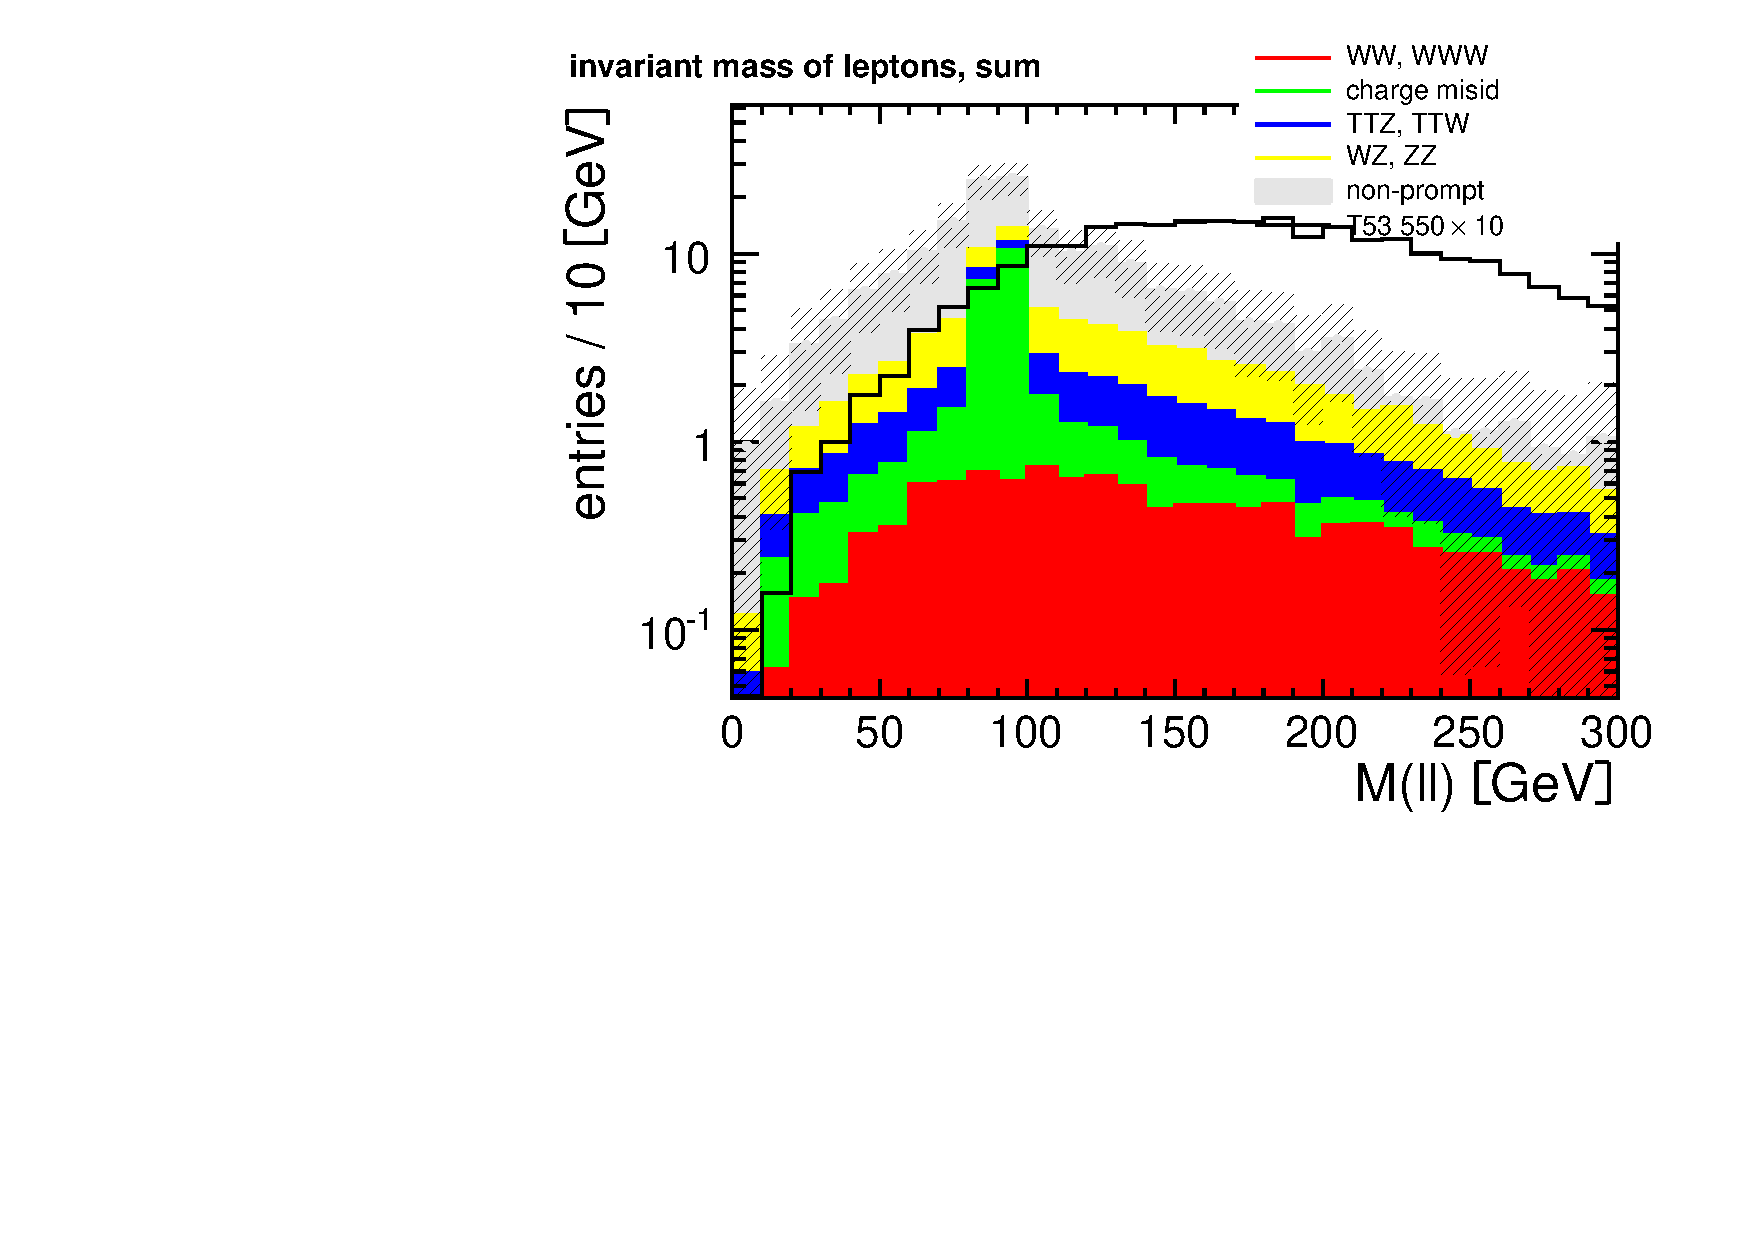
\includegraphics[width=.7\textwidth]{images/pdf/same-sign,_2_jets/lep_mass_sum_0}
    \caption{Events with two same-sign leptons and two jets. Distribution of the invariant mass of the leptons in the backgrounds and
        signal for the \unit[550]{GeV} mass point for the sum of the three
        decay channels \E\E, \E\M\ and \M\M, and their sum. The signal is
    amplified by factor of ten, the data-driven backgrounds for the
non-prompt and charge misidentification contributions are detailed in
chapter~\ref{chap:data_driven}. The shaded area includes statistical and
systematic uncertainties.}
    \label{fig:lep_mass}
\end{figure}
While the prompt same-sign background is well modelled by the Monte Carlo, we
found that a data-driven method is needed for an accurate description of the
contributions from charge misidentification and non-prompt leptons.
That is the subject of the following chapter.
